\documentclass[12pt,a4paper]{article}
\usepackage[colorlinks=true, urlcolor=blue, linkcolor=red]{hyperref}
\usepackage{amsmath, amssymb, amsthm, algorithm, booktabs, listings}
\usepackage[dvipsnames,usenames]{xcolor}
\usepackage[noend]{algpseudocode}
\usepackage{tikz}
\usepackage{fancyhdr}
\usepackage{geometry}
\newgeometry{top=2cm, bottom=2cm, left=1.5cm, right=1.5cm}
\usepackage[shortlabels]{enumitem}
\usepackage{cleveref}
\usepackage{mdframed}
\usepackage[most]{tcolorbox}
\hypersetup{citecolor=blue}
\usepackage{times}
\theoremstyle{definition}
\newtheorem{definition}{Definition}[subsection]
\newtheorem{statement}{Statement}[subsection]
\usepackage[backend=biber,style=alphabetic,sorting=ynt]{biblatex}
\hypersetup{linkcolor=black}
\addbibresource{references.bib}
\pagestyle{fancy}
\defbibheading{blueboxed}{%
  \begin{tcolorbox}[colframe=blue!50!black, colback=blue!20]
    \section{References}
  \end{tcolorbox}
}

\newcommand{\bluebox}[1]{%
  \begin{tcolorbox}[colframe=blue!50!black, colback=blue!20]
    #1
  \end{tcolorbox}%
}

\newcommand{\purplebox}[1]{%
  \begin{tcolorbox}[colframe=violet!80!black, colback=violet!20]
    #1
  \end{tcolorbox}%
}

\newcommand{\pinkbox}[2]{%
  \begin{tcolorbox}[colframe=magenta!50!black, colback=magenta!20, title={#1}]
    #2
  \end{tcolorbox}%
}

\newcommand{\bluebigbox}[2]{%
  \begin{tcolorbox}[colframe=blue!50!black, colback=blue!20, title={#1}, toptitle=5pt, bottomtitle=5pt]
    #2
  \end{tcolorbox}%
}

\DeclareRobustCommand{\hlit}[1]{\colorbox{yellow}{\textit{#1}}}
\DeclareRobustCommand{\hl}[1]{\colorbox{yellow}{#1}}
\DeclareRobustCommand{\ghl}[1]{\colorbox{green}{#1}}
\newcommand{\bs}{\textbackslash}
\newcommand{\boxtxt}[1]{\boxed{\text{#1}}}

\tcbuselibrary{listings}
\newtcblisting{shuncode}{
    listing only,
    listing options={
        language=C,
        basicstyle=\ttfamily\small,
        keywordstyle=\color{blue},
        commentstyle=\color{green!50!black},
        stringstyle=\color{red}
    },
    colback=cyan!10,
    colframe=cyan!80!black,
    boxrule=2pt,
    left=0pt,
    right=0pt,
    top=0pt,
    bottom=0pt,
    boxsep=0pt,
    arc=5pt,
    enhanced
}

\lhead{Computer Networks}
\chead{Chapter 2 Summary}
\rhead{Shun (@shun4midx)}

\begin{document}
\begin{center}
  {\Large \bf Computer Networks: Chapter 2 Summary}\\[8pt]
  \textbf{Author:} Shun (@shun4midx)
\end{center}

\bluesec{Principles of Network Applications}

\noindent The key idea is to enable programs to be able to run on \textbf{different end systems} --- network-core devices \textbf{do not run user applications}. \\

\purplesec{Client-Server Paradigm}

\noindent Here, we divide communication into two types of entities:

\vspace{0.5em}\begin{itemize}
  \item \textbf{Server:} \hl{\textbf{Always-on} host, \textbf{permanent IP} address}, \textit{often in data centers}
  \item \textbf{Clients:} \textit{Communicate with server}, may be intermittently connected, may have dynamic IP addresses, \hlbf{do not communicate directly with each other}
\end{itemize}

\noindent Some examples of \hl{client-server paradigm are: \textit{HTTP, IMAP, FTP}} \\

\purplesec{Peer-Peer (P2P) Architecture}

\begin{itemize}
  \item \textbf{No always-on server}: \textbf{arbitrary end systems} directly communicate
  \item Peers request service from other peers, and provide service in return to other peers

  $\Rightarrow$ \hl{\textbf{Self scalability} -- new peers bring \textbf{new service capacity and demands}}

  \item Peers are \textit{intermittently connected} and \textit{change IP addresses}
\end{itemize}

\noindent An example of this is \hlit{P2P file sharing}. \\

\purplesec{Process Communication and Addressing}

\pinkbox{Definition of Processes}{
  A \textbf{process} is a \textit{program} running within a \textit{host}.
  \begin{itemize}
    \item Within the \textit{\textbf{same host}}, two processes communicate using \textbf{inter-process communication}
    \item Between \textit{\textbf{different hosts}}, they communicate by exchanging \textbf{messages}
    \item \textbf{Client Process:} A process that \textit{\textbf{initiates} communication}
    \item \textbf{Server Process:} A process that \textit{\textbf{waits} to be contacted}
  \end{itemize}

  P2P applications still have client and server processes, despite not having clients or servers.
}

\pinkbox{Sockets}{
  A process \textit{sends or receives} messages to or from its \textbf{socket}. In between a sending and receiving socket, we require some \hlbf{transport infrastructure}.
}

\pinkbox{Addressing Processes}{
  We need an \textbf{identifier} to receive addresses, which includes both the \textbf{(unique 32-bit) IP address} and \textbf{port numbers} needed for the process (since the same host may run many different processes).
}

\vspace{1.0em}
\purplesec{Transport-Layer Services}

\pinkbox{Application-Layer Protocol}{
  An \hlbf{application-layer protocol} defines:
  \begin{itemize}
    \item \textbf{Types of messages exchanged} (e.g. request, response)
    \item \textbf{Message Syntax}
    \item \textbf{Message Semantics} (i.e. meaning of information in fields)
    \item \textbf{Rules} for when to \textbf{send and respond} to messages
  \end{itemize}

  \noindent Examples of \textbf{open protocols} are \textit{HTTP, SMTP}. Examples of \textbf{proprietary protocols} are \textit{Skype, Zoom}.
}

\pinkbox{TCP vs UDP Services}{
  TCP and UDP services can almost be seen as polar opposites:
  \begin{itemize}
    \item \hl{\textbf{TCP:} \textbf{Reliable transport} \textit{flow control, congestion control} (throttle sender when network} \hl{overloaded), connection-oriented \textbf{(setup required between client and server processes)}}
    \item \textbf{TCP doesn't provide:} Timing, minimum throughput guarantee, security
    \item \hl{\textbf{UDP:} \textbf{Unreliable data transfer} (may be not received), but typically \textbf{faster speeds}}
    \item \textbf{UDP doesn't provide:} What TCP doesn't + what TCP does
  \end{itemize}

  \noindent Most applications want to use TCP, but interactive games and Internet telephony may use UDP.
}

\pinkbox{Transport Layer Security}{
  \textbf{Transport Layer Security (TLS)} provides \textbf{encrypted} TCP connections and end-point authentication, since otherwise passwords are sent in plain text. It is implemented in the \textbf{application layer}.
}

\vspace{1.0em}
\bluesec{Web and HTTP (HyperText Transfer Protocol)}

\purplesec{Overview}

\noindent\textbf{HTTP} is the web's \hlit{application-layer protocol} that uses the client/server model, where: \\

\begin{itemize}
  \item \textbf{Client:} Browser that requests/receives (using HTTP protocol), and displays web objects
  \item \textbf{Server:} Web server sends (using HTTP protocol) objects in response to the requests
\end{itemize}

\noindent\hlbf{HTTP uses TCP} and does it in basically the following steps:
\begin{itemize}
  \item The client \textbf{initiates TCP connection} (creates a \textbf{socket}) to the server at \textbf{port 80}
  \item The server \textbf{accepts TCP connection} from the client
  \item HTTP messages are exchanged between the browser (HTTP client) and Web server (HTTP server)
  \item \textbf{TCP connection closed}
\end{itemize}

\noindent \hl{Note, HTTP is \textbf{stateless} -- the server maintains \textbf{no information about past client requests}}. \\

\purplesec{HTTP Connections: Persistent vs Non-Persistent}

\pinkbox{Persistent vs Non-Persistent HTTP Connections}{
  \renewcommand{\arraystretch}{1.1}
  \setlength{\tabcolsep}{10pt}

  \begin{center}
    \begin{tabular}[t]{@{}p{0.46\textwidth}|p{0.46\textwidth}@{}}
  \multicolumn{1}{c}{\textbf{Non-Persistent HTTP}} &
  \multicolumn{1}{c}{\textbf{Persistent HTTP}} \\[0.5em]
  \hline\\[-1.0em]
  \begin{minipage}[t]{\linewidth}
    \begin{enumerate}[leftmargin=*, topsep=0pt, itemsep=0.5em]
      \item TCP connection opened
      \item \textbf{At most one object} sent over TCP connection
      \item TCP connection closed
    \end{enumerate}
  \end{minipage}
  &
  \begin{minipage}[t]{\linewidth}
    \begin{enumerate}[leftmargin=*, topsep=0pt, itemsep=0.5em]
      \item TCP connection opened to a server
      \item \textbf{Multiple objects} can be sent over a TCP connection between client and that server
      \item TCP connection closed
    \end{enumerate}
  \end{minipage}
  \\
  \end{tabular}
  \end{center}

  \vspace{0.5em}\hl{For non-persistent HTTP, downloading \textbf{multiple objects requires multiple connections.}}
}

\pinkbox{RTT}{
  \textbf{RTT} is the time for a small packet to \textbf{travel from client to server and back}.
}

\pinkbox{HTTP Response Time Per Object}{
  % Fill for nonpersistent vs persistent
  For \textbf{non-persistent HTTP}, the HTTP response time \textbf{per object} is: \\
  
  {\centering
  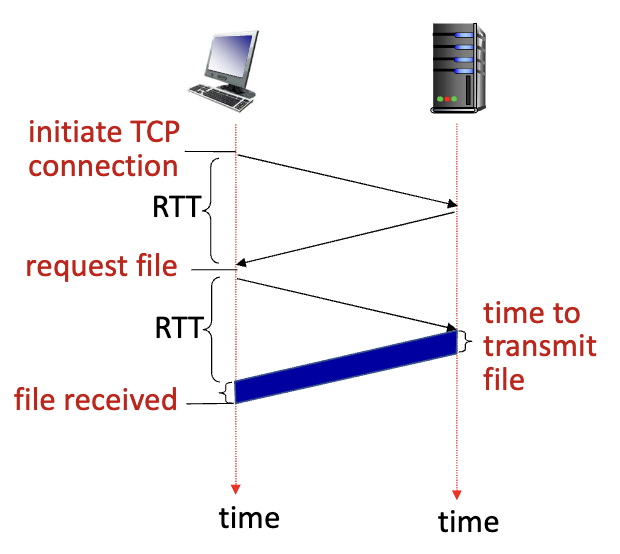
\includegraphics[width=0.35\textwidth]{ch2_img/nonpersistent_rtt.png}
  \par
  }
  
  \vspace{1.0em}Hence, \hl{\boxed{\text{\textbf{Non-persistent PER OBJECT} HTTP response time = \textbf{2RTT + File transmisison time}}}} \\

  Similarly, for \textbf{persistent HTTP}, instead of per object, we can transmit multiple files, hence \hl{\boxed{\text{\textbf{Persistent TOTAL} HTTP response time = \textbf{2RTT + ALL files transmission time}}}}
}

\vspace{1.0em}\purplesec{HTTP Request Messages}

\pinkbox{General Format}{
  The image below provides the typical body of an HTTP request message. \\

  Usually in the request line, the method is in all caps, such as \hlit{GET, POST, HEAD, PUT}. \\

  \texttt{cr} and \texttt{lf} refer to \textbf{carriage return character} and \textbf{line-feed character} respectively, typically denoted as \texttt{\bs r} and \texttt{\bs f}. \\

  \hl{A \textbf{blank line (CRLF CRLF)} indicates the \textbf{end of the header section}, not the entire message.} The optional \textbf{entity body} follows this blank line. \\

  {\centering
  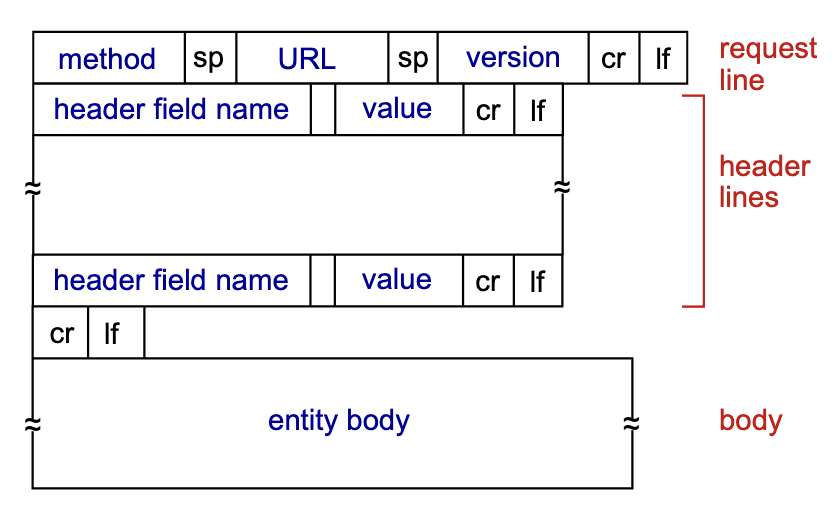
\includegraphics[width=0.5\textwidth]{ch2_img/html_request.png}
  \par
  }
}

\pinkbox{Details About HTTP Request Message Methods}{
  There are four main message methods:

  \begin{itemize}
    \item \textbf{POST:} Web page includes \textbf{form input}, with the user input sent from client to server in the \textbf{body of a HTTP POST} request
    \item \textbf{GET:} It \textbf{sends data to a server}, oftentimes including \textbf{user data in the URL field} of a HTTP GET request message \textbf{following a '\texttt{?}'}
    \item \textbf{HEAD:} \textbf{Requests headers} that would be returned \textbf{if} the URL were requested with HTTP GET
    \item \textbf{PUT:} \textbf{Uploads a new file} to the server, and completely \textbf{replaces the file} that exists at the URL with content in the \textbf{body of a HTTP PUT} request
  \end{itemize}
}

\begin{shuncmd}[Example of a Real HTTP Request Message]
  GET /index.html HTTP/1.1 \r\n
  Host: www.example.com \r\n
  User-Agent: Chrome/133.0 \r\n
  Accept-Language: en-US \r\n
  \r\n
  <body>
  \r\n
\end{shuncmd}

\purplesec{HTTP Response Messages}

\pinkbox{General Format}{
  \texttt{<protocol><status code>} 

  \texttt{<header lines>}
 
  \texttt{<blank line>}
 
  \texttt{<optional entity body>}
}

\pinkbox{HTTP Response Status Codes}{
  The \textbf{status code} is what appears in the first line in the server-to-client response message. Here are some common sample codes:

  \begin{itemize}
    \item \textbf{200 OK:} Request \textbf{succeeded}, requested object later in this message
    \item \textbf{301 Moved Permanently:} Requested \textbf{object moved}, new location specified later in this message (in \texttt{Location:} \texttt{field})
    \item \textbf{400 Bad Request:} Request message \textbf{not understood by server}
    \item \textbf{404 Not Found:} Requested document \textbf{not found} on this server
    \item \textbf{505 HTTP Version Not Supported}
  \end{itemize}
}

\begin{shuncmd}[Example of a Real HTTP Response Message]
  HTTP/1.1 200 OK\r\n
  Date: Fri, 17 Oct 2025 07:00:00 GMT\r\n
  Server: Apache/2.4\r\n
  Content-Type: text/html\r\n
  Content-Length: 512\r\n
  \r\n
  <html>...</html>
\end{shuncmd}  

\vspace{1.0em}\purplesec{Cookies}

\noindent Recall that the HTTP GET/response interaction is \textbf{stateless}. In order to maintain some states between transactions, websites and client browsers use \textbf{cookies}. To maintain cookies, we need four main components: \\

\begin{itemize}
  \item Cookie header line in \textbf{HTTP response} message
  \item Cookie header line in \textbf{next HTTP request} message
  \item Cookie file kept on \textbf{user's host} (managed by user's browser)
  \item Backend \textbf{database at website}
\end{itemize}

\noindent They are typically used for \hlit{authorization, shopping carts, or ad recommendations}. Third party cookies (persistent cookies) allow for the same cookie value to be tracked across multiple websites, which is an invasion of privacy.

\noindent The following image below shows how cookies are maintained:
\begin{figure}[h]
  \centering
  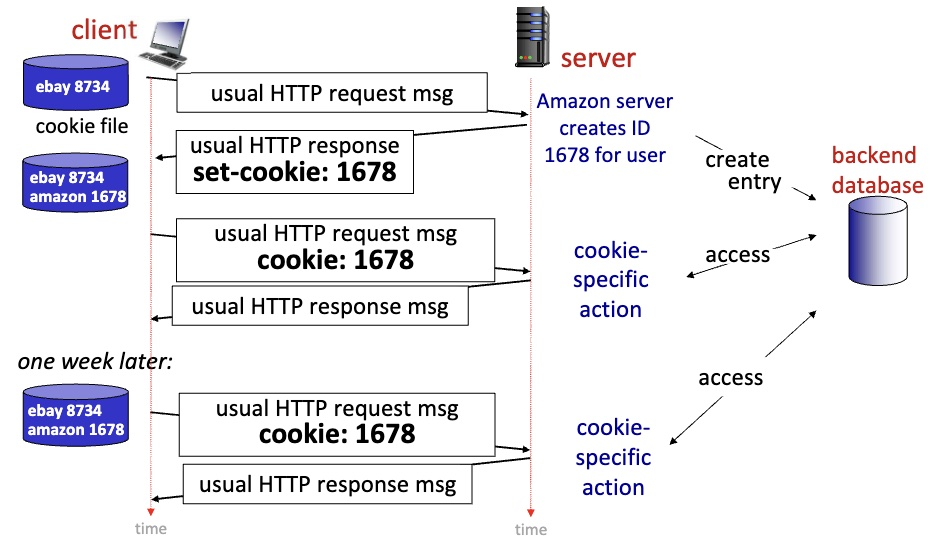
\includegraphics[width=0.6\textwidth]{ch2_img/cookies.jpg}
\end{figure}

\bluesec{Web Caches (i.e. Proxy Servers)}

\pinkbox{Goal}{To satisfy client requests without requesting from the origin server, which helps reduce response time and \textbf{traffic on an institution's access link}}

\pinkbox{Implementation}{
  We have the user's broswer point to a \textbf{web cache}, then have the browser send all HTTPs to the web cache only. \textit{(More specifically, if the object is in the cache, the cache returns the object directly to the client. Else, it requests the object from the origin server, caches the object, then returns the object to the client.)} \\

  The server tells cache about the object's allowed caching in the response header as either of the two: 

  \begin{itemize}
    \item \texttt{Cache-Control: max-age=<seconds>}
    \item \texttt{Cache-Control: no-cache}
  \end{itemize}

  Thus, the web cache acts \hlbf{both as a client (to origin) and a server (to users)}.
}

\pinkbox{Calculation}{
  Typically, the \boxed{\text{End-end delay = Internet delay + Access link delay + LAN delay}} , where the LAN delay is typically in microseconds. \\

  What \textbf{caching minimizes is the number of times the access link is used}, which thus minimizes access link delay.
}

\pinkbox{Conditional GET}{
  \textbf{Goal:} Don't send object if cache has up-to-date cached version, to reduce object transmission delay. \\

  To do so, we maintain the following:

  \begin{itemize}
    \item \textbf{Client:} Store date of cached copy in HTTP request via \hl{\texttt{if-modified-since:} \texttt{<date>}}
    \item \textbf{Server:} If cached copy is up-to-date, don't return an object, and send status code \hlbf{\texttt{HTTP/1.0 304 Not Modified}}. Otherwise, do a \textit{normal HTTP GET request}.
  \end{itemize}
}

\vspace{1.0em}\bluesec{HTTP/2 and HTTP/3}

\pinkbox{Key Goal}{
  \textbf{Decrease delay} in \textbf{multi-object} HTTP requests.
}

\purplesec{HTTP/1.1}
\noindent Introduced \textbf{multiple, pipelined GETs} over a \textit{single TCP connection} \\

\begin{itemize}
  \item Server responds \hlbf{in-order FCFS (First Come First Serve)} to GET requests
  \item With FCFS, small objects may have to \hlbf{wait for transmission behind large objects} (which is known as \textbf{HOL, i.e. head-of-line, blocking})
  \item Loss recovery (retransmitting lost TCP segments) stalls object transmission
\end{itemize}

\purplesec{HTTP/2}

\noindent HTTP/2 increased flexibility at server in sending objects to client: \\
\begin{itemize}
  \item Transmission order of requested objects based on \textit{client-specified object priority} (may not be FCFS)
  \item Push unrequested objects to the client
  \item Divide objects into ``frames'', and \hlbf{schedule frames to mitigate HOL blocking}, as shown below
\end{itemize}

\vspace{-1.0em}\begin{figure}[h]
  \centering
  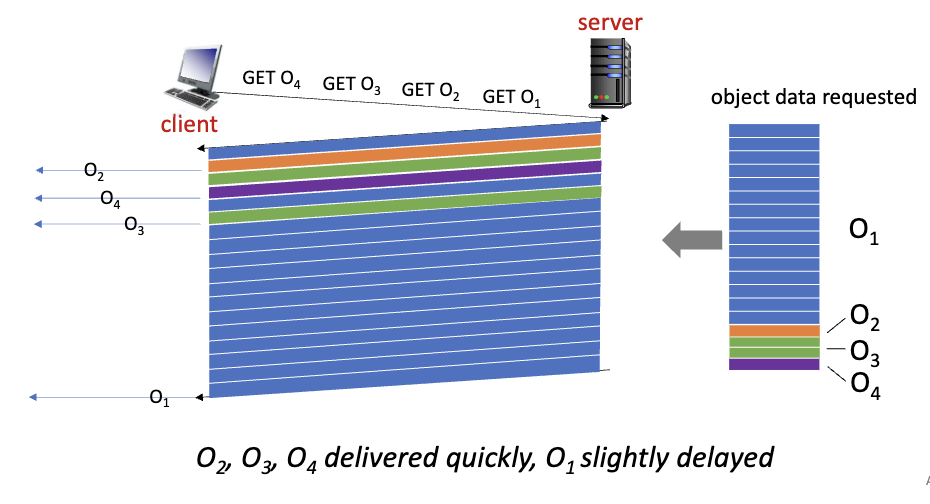
\includegraphics[width=0.6\textwidth]{ch2_img/http2.png}
\end{figure}

\purplesec{HTTP/3}

\noindent HTTP/2 over a single TCP connection means \textbf{recovery from packet loss} still \hl{stalls all object transmissions} \\

\noindent HTTP/3 added \textbf{security} over vanilla TCP connection and \textbf{per object error-control and congestion-control} over UDP (hence minimizing packet loss recovery).

\vspace{1.0em}\bluesec{E-Mail, SMTP, IMAP}

\purplesec{Components}

\noindent There are three major components: \\

\begin{itemize}
  \item \textbf{User agents:} The ``mail reader'' used to compose, edit, and read mail messages (such as \textit{Gmail, Outlook, mail client})
  \item \textbf{Mail servers:} We have the \textbf{mailbox containing incoming messages} for the user, and \textbf{message queue of outgoing} (to be sent) mail messages
  \item \textbf{Simple Mail Transfer (SMTP) Protocol:} Used between mail servers to send email messages, with the \textit{``client'' being the sending mail server, and ``server'' being the receiving mail server}
\end{itemize}

\purplesec{SMTP RFC 5321 (SMTP Protocol)}
\noindent The SMTP uses TCP to \textit{reliably} transfer email message from client (mail server initiating connection) to server at \textbf{port 25} via command/response interaction like HTTP. \\

\noindent There are three phases of transfer (as also shown in the image below): \\

\vspace{-0.5em}\begin{enumerate}
  \item SMTP \textbf{handshaking}
  \item SMTP \textbf{transfer of messages}
  \item SMTP \textbf{closure}
\end{enumerate}

\vspace{-1.5em}\begin{figure}[h]
  \centering
  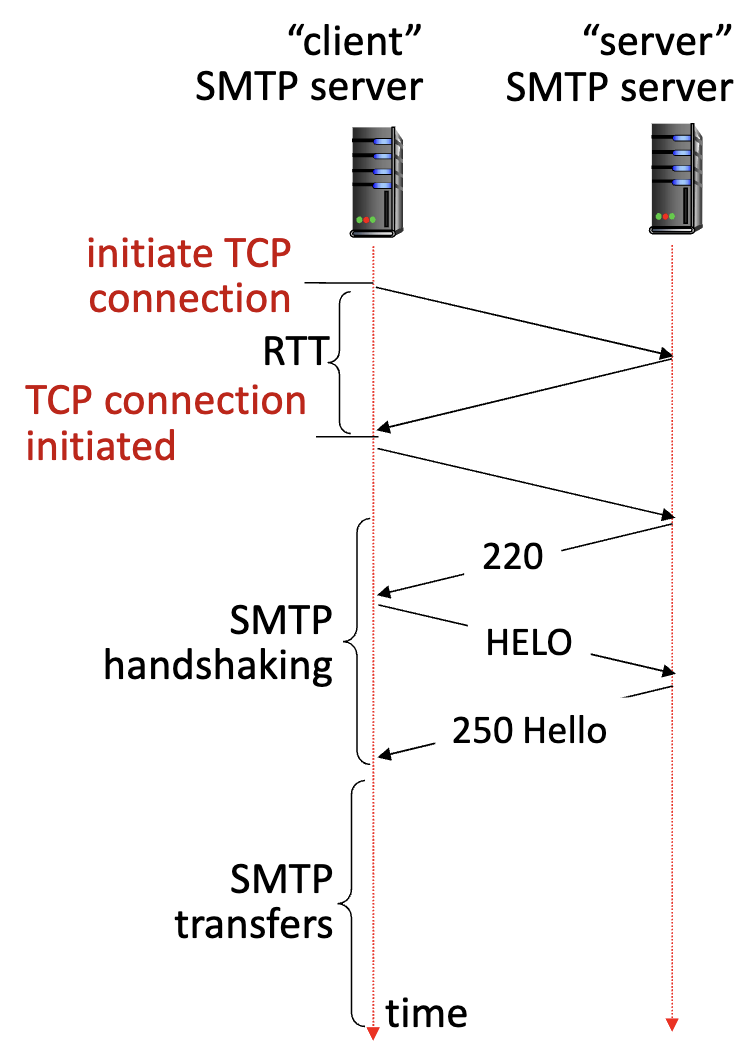
\includegraphics[width=0.3\textwidth]{ch2_img/smtp.png}
\end{figure}

\purplesec{SMTP Messages}

\begin{shuncmd}[Example SMTP Interaction]
S: 220 hamburger.edu
"C: HELO crepes.fr"
S: 250 Hello crepes.fr, pleased to meet you
"C: MAIL FROM: <alice@crepes.fr>"
S: 250 alice@crepes.fr... Sender ok
"C: RCPT TO: <bob@hamburger.edu>"
S: 250 bob@hamburger.edu... Recipient ok
C: DATA
S: 354 Enter mail, end with "." on a line by itself
C: Do you like ketchup?
C: How about pickles?
C: .
S: 250 Message accepted for delivery
C: QUIT
S: 221 hamburger.edu closing connection
\end{shuncmd}

\pinkbox{Ending of a Message}{
  To end a message in SMTP, we use a line with only ``.''
}

\pinkbox{SMTP vs HTTP}{
  \hl{HTTP is client pull whereas SMTP is client push}. Both have ASCII commands/response interaction and status codes, but HTTP has \textbf{each object} encapsulated in its \textbf{own response message}, whereas SMTP sends \textbf{multiple objects} in a \textbf{multipart message}. Thus, \hlbf{SMTP uses persistent connections}.
}

\pinkbox{SMTP Mail Messsage Format (RFC 2822)}{
  \centering
  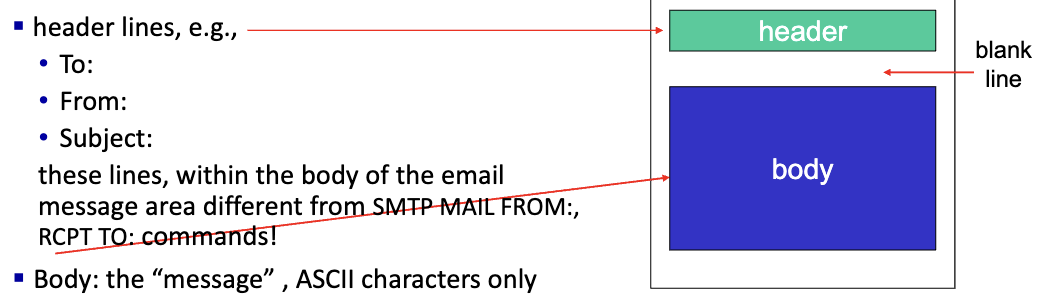
\includegraphics[width=\textwidth]{ch2_img/smtp_msg.png}
}

\vspace{1.0em}\purplesec{Retrieval Protocols}

\noindent Notice, \hlbf{SMTP is to send emails} only, we need \hlbf{IMAP (Internet Mail Access Protocol) to retrieve emails}. In fact, \textbf{HTTP} provides web-based interface on top of SMTP and IMAP to form a full sending and receiving mail system.

\vspace{1.0em}\bluesec{Domain Name System (DNS)}

\noindent The \textbf{Domain Name System (DNS)} is a \textbf{distributed database} in the hierarchy of many name servers. DNS servers communicate to resolve names (\hlbf{hostname-to-IP translation}) via \textbf{mappings}, and thus appears often in \textit{application-layer protocols}. DNS also provides services such as \textbf{host or mail server aliasing}. \\

\noindent It tends to be physically \textbf{decentralized} because otherwise there will be too much traffic, and difficult maintance. This is especially because DNS needs to be \textit{reliable and secure}, as a backbone of the Internet. \\

\purplesec{DNS Server Types}

\noindent In fact, we can represent different types of DNS in a hierarchical database. Going from \textbf{top to down} based on proximity is how a corresponding IP address for an alias is found. As we can see, the servers are divided into four main types: \hlbf{root name, top-level domain (TLD), authoritative, and local servers}. Note, \hlbf{local DNS doesn't belong to the hierarchy below}

\begin{figure}[h]
  \centering
  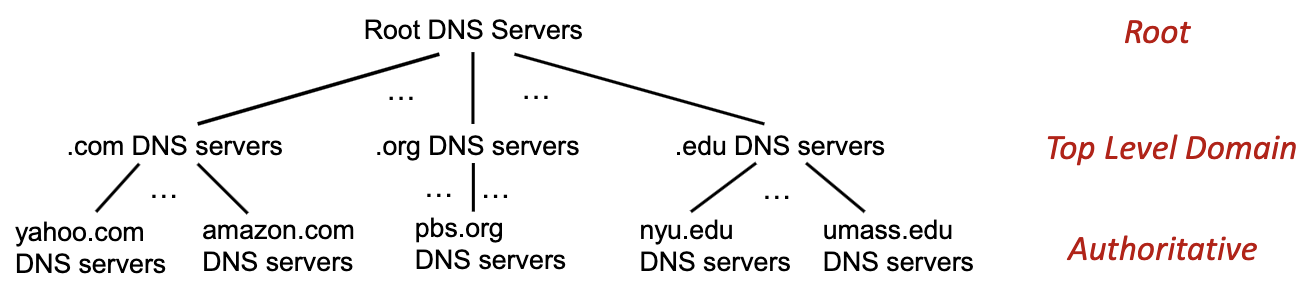
\includegraphics[width=0.9\textwidth]{ch2_img/dns_tree.png}
\end{figure}

\pinkbox{Root Name Servers}{
  They act the official \textbf{last resort} of any name servers that cannot resolve a domain name. Root name servers know where to \textbf{find the Top-Level Domain (TLD)} servers and help initiate the DNS resolution process. There are 13 worldwide root name servers, managed by the ICANN (Internet Corporation for Assigned Names and Numbers).
}

\pinkbox{Top-Level Domain (TLD) Servers}{
  Responsible for \textbf{\texttt{.com}, \texttt{.org}, \texttt{.net}, \texttt{.edu}, \texttt{.aero}, \texttt{.jobs}, \texttt{.museums}} and all \textbf{top-level country domains}, such as \texttt{.ca}, \texttt{.uk}, \texttt{.fr}, etc. They redirect you to the authoritative server.

  \begin{itemize}
    \item \textbf{Network Solutions:} Manages \textbf{\texttt{.com} and \texttt{.net}} TLDs.
    \item \textbf{EDUCAUSE:} Manages \textbf{\texttt{.edu}} TLD, used by educational institutions.
  \end{itemize}
}

\pinkbox{Authoritative Servers}{
  These are the \textbf{organization's own DNS servers}, providing authoritative hostname to IP mappings for organization's named hosts. They are maintained by the organization or service provider.
}

\pinkbox{Local Servers}{
  When a host makes a DNS query, it is sent to the local DNS server. The local DNS first answers by returning from its \textbf{local cache, and if unavailable, forwards request into the DNS hierarchy}. Each ISP has its own local DNS name server.
}

\purplesec{DNS Name Resolution: Iterated vs Recursive Query}

\noindent \hl{\textbf{Iterated query} is like \textbf{``I don't know this name but I'll recommend someone who does''}}, whereas \\ \hl{\textbf{recursive query} is like \textbf{``I don't know this name, but I'll ask someone who does then get back to you''}.}

\begin{figure}[h]
  \centering
  \begin{subfigure}[t]{0.48\textwidth}
    \centering
    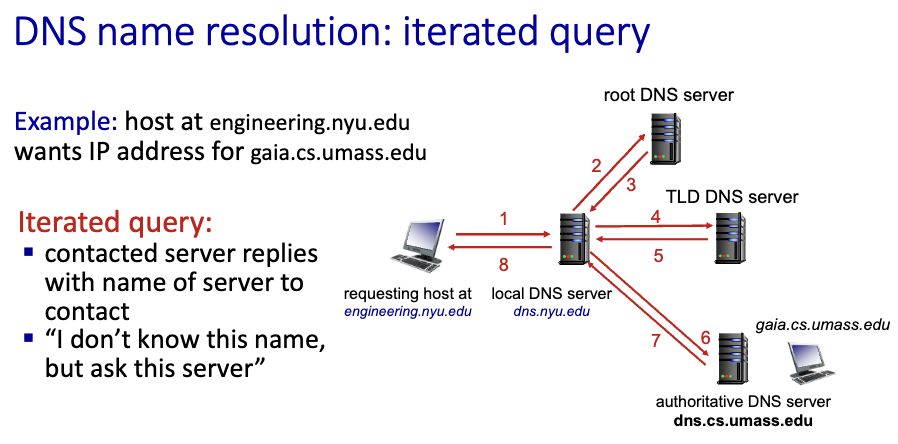
\includegraphics[width=\textwidth]{ch2_img/iterated_query.png}
  \end{subfigure}
  \hfill
  \begin{subfigure}[t]{0.48\textwidth}
    \centering
    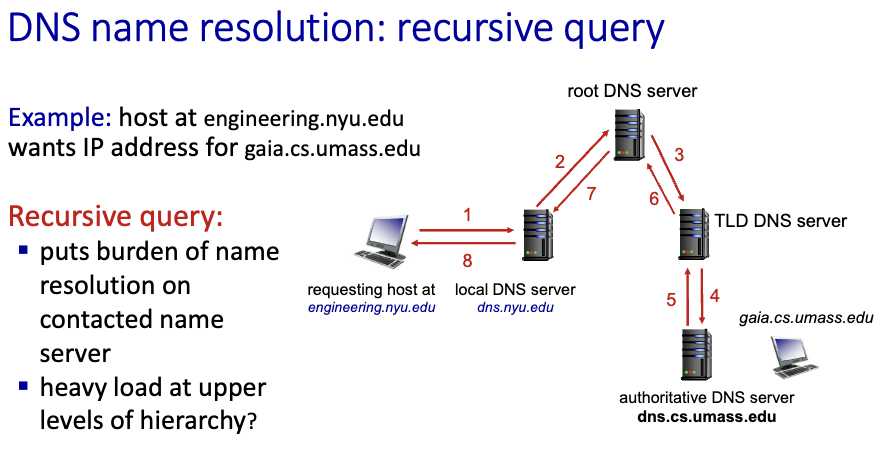
\includegraphics[width=\textwidth]{ch2_img/recursive_query.png}
  \end{subfigure}
\end{figure}

\purplesec{Caching Information}

\noindent Once a name server learns a mapping, it caches it, so that it can \textbf{immediately return} a cached mapping in response to a query, until its entry timeouts after some time---\textbf{Time to Live (TTL)}. TLD servers are typically cached in \textbf{local name servers}. However, cached entries may be \textbf{out-of-date}. If a named host changes its IP address, it may not be known Internet-wide until all TTLs expire. \\

\purplesec{DNS Records}

\noindent \textbf{Resource Records (RR)} are a distributed database, whose entries are \textbf{(\texttt{name}, \texttt{value}, \texttt{type}, \texttt{ttl})}. We type \hlbf{\texttt{nslookup}} in order to access the following:

\begin{itemize}
  \item \textbf{\texttt{type=A}}: \texttt{name} = \textbf{hostname}, \texttt{value} = \textbf{IP address}
  \item \textbf{\texttt{type=NS}}: \texttt{name} = \textbf{domain} (e.g. \texttt{.com}), \texttt{value} = hostname of \textbf{domain's authoritative name server}
  \item \textbf{\texttt{type=CNAME}}: \texttt{name} = \textbf{alias name} for some ``canonical'' (real) name, \texttt{value} = \textbf{canonical name}
  \item \textbf{\texttt{type=MX}}: \texttt{value} = name of \textbf{SMTP mail server} associated with \texttt{name}
\end{itemize}

\purplesec{DNS Message Format}

\noindent DNS query and reply messages both have the same format, as shown in the images below.

\begin{figure}[h]
  \centering
  \begin{subfigure}[t]{0.48\textwidth}
    \centering
    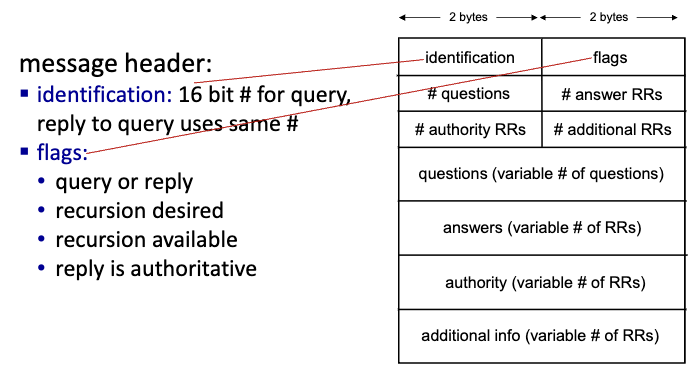
\includegraphics[width=\textwidth]{ch2_img/dns_msg1.png}
  \end{subfigure}
  \hfill
  \begin{subfigure}[t]{0.48\textwidth}
    \centering
    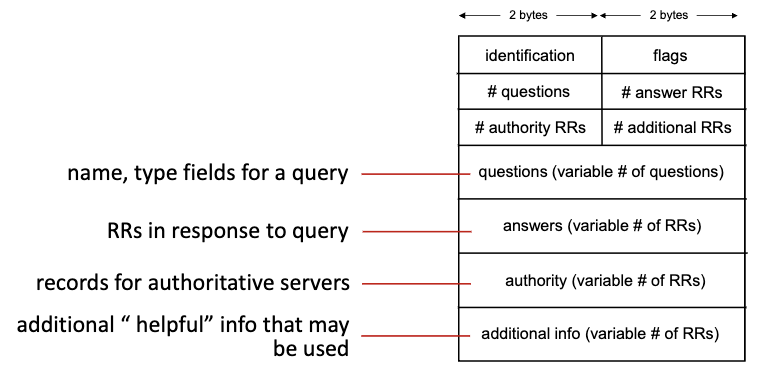
\includegraphics[width=\textwidth]{ch2_img/dns_msg2.png}
  \end{subfigure}
\end{figure}

\pinkbox{Example Setup for DNS}{
  Say you have a new startup called ``Network Utopia''. \\

  You must first create an \textbf{authoritative server locally}, perhaps with type \texttt{A} record at 
  
  \texttt{www.networkutopia.com} and type \texttt{MX} record for \texttt{networkutopia.com}. \\

  Then, you must first register a name, such as \texttt{networkutopia.com} at \textbf{DNS registrar} (e.g. Network Solutions). You'll have to provide \textbf{names and IP addresses of authoritative name server}, and the registrar will insert RRs of \textbf{types \texttt{NS} and \texttt{A}} into the \texttt{.com} TLD server.
}

\purplesec{Security}
\noindent One type of attacks are \textbf{DDoS (Distributed DoS) attacks}, which \textbf{bombard root servers with traffic}, so that they are not successful to date. They may also bombard TLD servers. \\

\noindent Another type of attacks are \textbf{spoofing attacks}, which intercept DNS queries and return \textbf{bogus replies}.

\vspace{1.0em}\bluesec{P2P Applications}

\purplesec{File Distribution Time: Client-Server vs P2P}

\pinkbox{File Distribution Example}{
  How much time does it take to distribute a file of \textbf{size} $\mathbf{F}$ from one server to $\mathbf{N}$ \textbf{peers}? 

  {
    \centering
    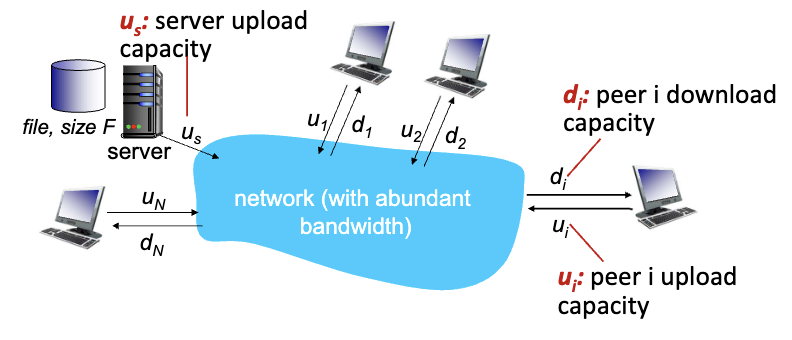
\includegraphics[width=0.6\textwidth]{ch2_img/file_distribution.png}
    \par
  }

  \vspace{1.0em}
  
  For \textbf{client-server}, the server transmission is done by sequentially sending $N$ file copies. The time it takes to send one copy is $\frac{F}{u_s}$, so the time it takes to send $N$ copies is $\frac{NF}{u_s}$. Each client must download one copy, so let $d_\text{min}$ be the minimum client download rate, then the maximum client download rate is $\frac{F}{d_\text{min}}$, so the total time taken is $\hl{\boxed{D_{c-s} \geq \max\{\frac{NF}{u_s}, \frac{F}{d_\text{min}}\}}}$. \\

  For \textbf{P2P}, the server must upload at least one copy, which takes time $\frac{F}{u_s}$. Each client must download a file copy, with maximum time $\frac{F}{d_\text{min}}$. Hence, all clients in total must download $NF$ bits, with limiting maximum upload rate as $u_s + \sum u_i$, i.e. both increase linearly in $N$. Thus, $\hl{\boxed{D_{P2P} \geq \max\{\frac{F}{u_s}, \frac{F}{d_\text{min}}, \frac{NF}{u_s + \sum u_i}\}}}$
}

\newpage

\noindent Here is an example of the difference between the time elapsed for client-server and P2P.

\begin{figure}[h]
  \centering
  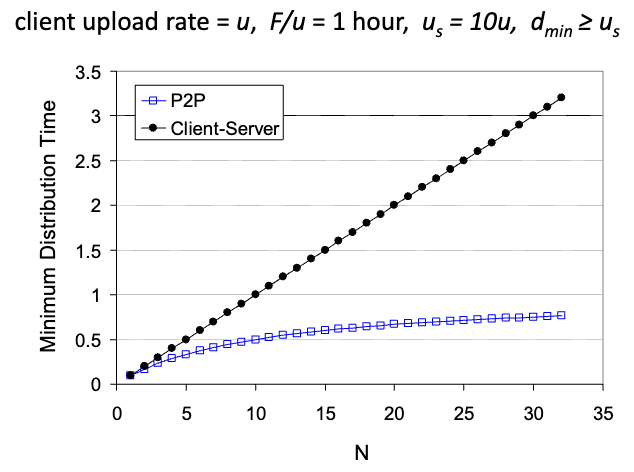
\includegraphics[width=0.5\textwidth]{ch2_img/client_p2p.png}
\end{figure}

\vspace{-2.0em}\purplesec{P2P File Distribution: BitTorrent}

\pinkbox{Overview}{
  BitTorrent is a type of P2P file distribution, where each file is divided into \textbf{256Kb chunks}. 

  \begin{itemize}
    \item \textbf{Torrent:} A group of peers exchanging chunks in a file
    \item \textbf{Tracker:} Tracks peers that participate in the torrent
  \end{itemize}

  When a peer joins a torrent, it has \textbf{no chunks}, but will \textbf{accumulate} them over time from other peers, and registers with tracker to get a list of peers, which connects it to neighbors. \\

  While downloading, the peer must upload chunks to other peers. Once the peer has the entire file, it may \hlbf{selfishly leave or altruistically remain} in torrent. We say that peers \textbf{``churn''}, meaning they may enter and leave the torrent.
}

\pinkbox{Requesting Chunks}{
  At any given time, different peers have different subsets of file chunks. Periodically, the user asks each peer for the list of chunks they have, they \textbf{request missing chunks from peers, rarest first}.
}

\pinkbox{Sending Chunks: Tit-For-Tat}{
  BitTorrent encourages fairness through a \textbf{Tit-for-Tat} strategy:

  \begin{itemize}
    \item Each peer \textbf{uploads to the four peers} that send to it at the \textbf{highest rate} (the ``unchoked'' peers)
    \item All other peers are \textbf{choked}, meaning they are temporarily denied uploads.
    \item Every 10 seconds, the peer re-evaluates which peers are its top four.
    \item Every 30 seconds, it \textbf{optimistically unchokes one random peer} to discover new partners.
  \end{itemize}

  \hl{Tit-for-tat resolves the issue of \textbf{free-riders (only downloading without uploading)}, by ensuring one} \hl{must upload before being able to download.}
}

\vspace{1.0em}\bluesec{Video Streaming and CDNs}

\purplesec{Multimedia: Video --- Terminology}

\begin{itemize}
  \item Video: A sequence of images displayed at a \textbf{constant rate}
  \item Digital Image: Array of pixels, each represented by bits
  \item \hl{\textbf{Coding:} Use \textbf{redundancy} within and between images to \textbf{decrease the number of bits used} to} \\ \hl{encode images}; \textit{spatial coding refers to it done withiin an image, and temporal coding refers to it done betweeen one image and the next}
  \item \textbf{Constant Bit Rate (CBR):} Video encoding rate is fixed
  \item \textbf{Variable Bit Rate (VBR):} Video encoding rate changes according to \textit{spatial and temporal coding}
\end{itemize}

\purplesec{Streaming Stored Video}

\pinkbox{Streaming vs Downloading}{
  \hl{Goal: Continuous playback despite network delay and rate variation.}

  \begin{itemize}
    \item \textbf{Stored video:} File pre-recorded and stored at the server.
    \item \textbf{Streaming:} Client begins playback before the entire file is downloaded.
    \item \hl{\textbf{Client Buffer:} Stores several seconds of video to handle delay and jitter, so it plays smoother} \hl{without having to have a fixed bitrate.}
  \end{itemize}
}

\vspace{-1.0em}\begin{figure}[h]
  \centering
  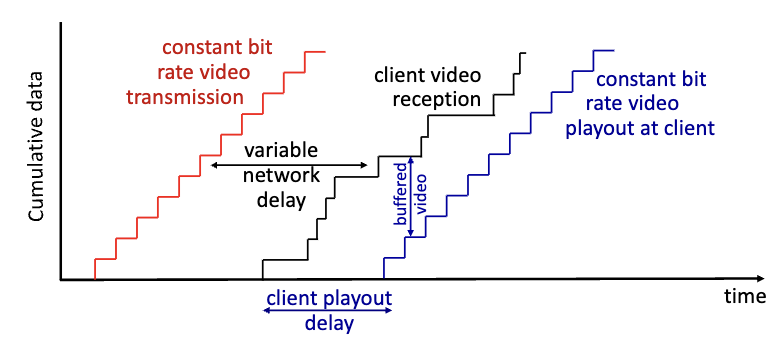
\includegraphics[width=0.7\textwidth]{ch2_img/streaming.png}
\end{figure}

\newpage

\purplesec{Streaming Multimedia: DASH}

\pinkbox{DASH: Dynamic Adaptive Streaming over HTTP}{
  \begin{itemize}
    \item Video file encoded into several versions with \textbf{different bitrates}.
    \item Each version is divided into \textbf{small chunks} (e.g. 2–10 seconds).
    \item \textbf{Manifest File:} Lists available bitrates and chunk URLs.
    \item \textbf{Client behavior:} 
      \begin{itemize}
        \item Downloads the manifest.
        \item Measures available bandwidth.
        \item Requests next chunk at the highest bitrate it can handle.
      \end{itemize}
  \end{itemize}

  \hl{Advantage: \textbf{Adapts to changing network conditions} to avoid stalls.}
}

\purplesec{Content Distribution Networks (CDNs)}

\pinkbox{Overview}{
  A CDN \hlbf{distributes copies of content across geographically separated servers} to reduce latency and server load.

  \begin{itemize}
    \item \hl{\textbf{Enter Deep (Type 1):} CDN servers \textbf{placed inside ISPs}}, close to users (e.g. Akamai).
    \item \hl{\textbf{Bring Home (Type 2):} CDN servers in a \textbf{few large data centers}} (e.g. Google, Netflix).
    \item \textbf{User Redirection:} DNS or HTTP redirects map clients to the nearest or least-loaded CDN node.
  \end{itemize}

  \hl{Goal: Reduce RTT, balance load, and minimize origin-server traffic.}
}

\vspace{1.0em}\bluesec{[NOTES MADE LATER] Socket Programming}

\noindent TBD!

\end{document}